\begin{document}
% Lecture Notes: Bioinformatics Algorithms: Hidden Markov Models for Sequence Modeling
\section{Introduction to Sequence Modeling}

When analyzing large, unlabelled chunks of DNA (such as parts of a newly sequenced genome), we typically want to identify functional regions: protein-coding genes, regulatory motifs, or structural elements. While simple string matching (e.g., searching for the "ATG" start codon) might seem intuitive, it is insufficient because such short patterns appear randomly with high frequency across the genome.

Bioinformatics relies on sophisticated models to extract signal from this biological noise. Biological data is inherently noisy due to natural variation, evolutionary experimentation, and sequencing errors. Therefore, probabilistic models are preferred over rigid, deterministic rules, as they provide a calculus for manipulating uncertainty and return "degrees of belief" rather than binary yes/no answers.

\begin{important}
  \textbf{Goals of Probabilistic Sequence Modeling:}
  \begin{itemize}
      \item \textbf{Emit/Generate:} The ability to generate random DNA sequences that respect the statistical properties of a certain biological type (e.g., simulating promoters).
      \item \textbf{Recognize/Decode:} The ability to determine the most likely hidden functional state (e.g., exon, intron, intergenic) that generated a given observed sequence.
      \item \textbf{Learn:} The ability to train generative models on large datasets to learn distinguishing characteristics and classify unlabelled data.
  \end{itemize}
\end{important}

While alignment profiles or motifs serve as basic models for specific DNA patterns (like transcription factor binding sites), they assume all instances of the pattern have the same fixed length. Functional genomic elements, such as CpG islands or protein-coding genes, vary wildly in length due to different numbers of exons, varying intron sizes, and diverse encoded proteins. To model genomic regions of variable length, we utilize Markov Chains and Hidden Markov Models (HMMs).

\section{Markov Chains and Hidden Markov Models}

At the core of these probabilistic sequence models is the concept of a state machine transitioning over time, heavily relying on the memoryless property.

\begin{important}
  \textbf{Markov Chain}: A probabilistic model consisting of a finite set of states with defined transition probabilities between them.
  In a standard Markov Chain, the states themselves are the observable output.
\end{important}

\sta A critical property of Markov Chains is that they are \textit{memoryless}. The probability of transitioning to the next state depends exclusively on the current state, completely ignoring the historical path taken to arrive there:
\begin{equation}
  P(x_i \mid x_{i-1}, \dots, x_1) = P(x_i \mid x_{i-1})
\end{equation}

The total probability of observing a specific sequence of states $x$ of length $L$ is simply the product of the initial probability and all subsequent transition probabilities:
\[
  P(x) = P(x_L \mid x_{L-1}) \times P(x_{L-1} \mid x_{L-2}) \times \dots \times P(x_2 \mid x_1) \times P(x_1)
\]

In many real-world biological scenarios, the functional state of the DNA is not written directly into the sequence; it is hidden. We can only observe the nucleotide output (A, C, G, T) and must infer the state that generated it.

\begin{important}
  \textbf{Hidden Markov Model (HMM)}: A 5-tuple $(Q, V, p, A, E)$ where the underlying state transitions follow a Markov process, but the states are hidden. Instead, each state emits observable symbols according to specific emission probabilities.
  \begin{itemize}
      \item $Q$: A finite set of hidden states $q_n$ ($|Q| = N$).
      \item $V$: A finite set of observable symbols $v_m$ ($|V| = M$).
      \item $p$: A vector of initial state probabilities.
      \item $A$: The $N \times N$ matrix of state transition probabilities, $a_{kl} = P(\pi_i = l \mid \pi_{i-1} = k)$.
      \item $E$: The $N \times M$ matrix of emission probabilities, $e_k(v_m) = P(x_i = v_m \mid \pi_i = q_k)$.
  \end{itemize}
\end{important}

\sta In an HMM, \textbf{both} transitions and emissions are memoryless. The probability of emitting a symbol depends entirely on the current hidden state, not on previous emissions or states.

\textbf{Example:} Predicting the Weather.
If weather states (Sun, Rain, Clouds) transition directly and are observed, it is a standard Markov Chain. If the hidden states are the \textit{seasons} (Summer, Winter) and the observable outputs are the daily weather conditions (Sun, Snow), it is an HMM. You cannot directly observe "Summer", but a sequence of sunny days allows you to infer that the hidden state is likely Summer based on high emission probabilities for Sun during that state.

\subsection{The Dishonest Casino Example}

To understand how HMMs parse hidden information from observable sequences, consider a hypothetical casino that uses two types of dice.

\begin{center}
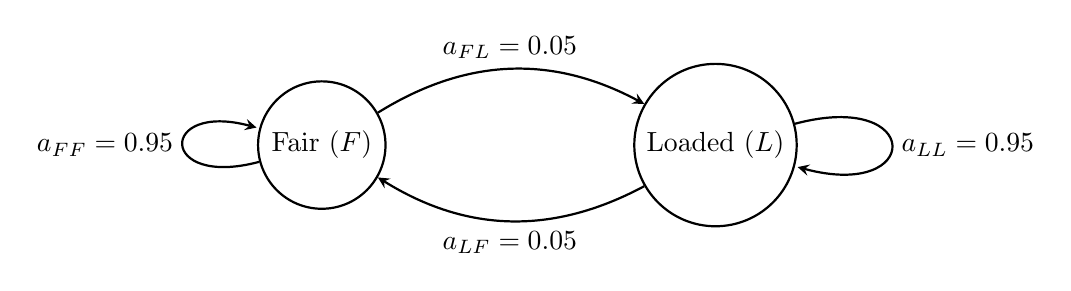
\begin{tikzpicture}[->, >=stealth, node distance=5cm, auto, thick]
    \node[circle, draw, minimum size=1.5cm] (F) {Fair ($F$)};
    \node[circle, draw, minimum size=1.5cm] (L) [right of=F] {Loaded ($L$)};

    \path
    (F) edge [loop left] node {$a_{FF} = 0.95$} (F)
        edge [bend left] node {$a_{FL} = 0.05$} (L)
    (L) edge [loop right] node {$a_{LL} = 0.95$} (L)
        edge [bend left] node {$a_{LF} = 0.05$} (F);
\end{tikzpicture}
\end{center}

\textbf{Example:} The Dishonest Casino.
The casino has a Fair die ($D_F$) where $P(1..6) = 1/6$, and a Loaded die ($D_L$) where $P(6) = 1/2$ and $P(1..5) = 1/10$. The dealer switches between the dice with a $5\%$ probability per turn.
\textit{This illustrates a two-state HMM where the choice of die is hidden, and the rolled numbers are the observable emissions.}

We want to know the probability of a specific sequence of hidden states (a hidden path $\pi$) jointly with a specific sequence of observations $x$. The joint probability is the product of the path probability and the emission probability given that path:
\[
  P(x, \pi) = P(x \mid \pi)P(\pi) = \prod_{i} e_{\pi_i}(x_i) \times \prod_{i} a_{\pi_{i-1}\pi_i}
\]

If we observe the rolls $x = (1, 2, 1, 5, 6, 2, 1, 6, 2, 4)$, we can evaluate specific hypothetical paths. Assuming an initial probability of $0.5$ for starting in either state:
\begin{align*}
  P(x, \text{all-Fair}) &= \frac{1}{2} \times \left(\frac{1}{6}\right)^{10} \times (0.95)^9 \approx 5.2 \times 10^{-9} \\
  P(x, \text{all-Loaded}) &= \frac{1}{2} \times \left(\frac{1}{10}\right)^8 \times \left(\frac{1}{2}\right)^2 \times (0.95)^9 \approx 7.9 \times 10^{-10}
\end{align*}
The all-Fair path is $6.59$ times more likely than the all-Loaded path for this particular sequence. However, if the sequence contained many more $6$s, the calculation would heavily favor the Loaded path due to its distinct emission probabilities.

This problem mimics the "Dishonest Genome," where a model must classify sequence regions as either Human (Background) or Viral (Integrated DNA). The hidden states govern the expected nucleotide frequencies, and transitions between them are rare but possible.

% [IMAGE: Header of the paper 'Prediction of Complete Gene Structures in Human Genomic DNA' by Burge and Karlin, introducing GENSCAN.]
% [IMAGE: Complex HMM architecture (GENSCAN) for predicting protein-coding genes, showing hidden states for UTRs, Exons, Introns, and start/stop/splice signals across different reading frames.]

\section{Algorithmic Settings for HMMs}

When working with HMMs, we are fundamentally trying to solve specific types of inferences. There are multiple algorithmic settings depending on whether we are optimizing over a single path or summing over all paths, and whether our goal is decoding, evaluation, or learning.

\subsection{Decoding: The Viterbi Algorithm (Most Likely Path)}

Given the model parameters (transitions $a$ and emissions $e$) and an observed sequence $x$, our goal is to find the single most likely sequence of hidden states $\pi^*$ that generated $x$.

Evaluating every possible path individually is computationally intractable due to the exponential number of path combinations. However, the problem exhibits \textit{optimal substructure}: the best path reaching state $k$ at step $i$ is strictly composed of the best path reaching some state $j$ at step $i-1$, followed by the transition from $j$ to $k$, and the emission of $x_i$ at $k$.

This allows us to use Dynamic Programming via the \textbf{Viterbi Algorithm}.

\begin{minted}{text}
# [pseudocode]
Input: Sequence of observations x = x_1 ... x_N
Initialization:
  V_0(0) = 1        # Start in a null state
  V_k(0) = 0        # For all k > 0
Iteration (for i = 1 to N):
  For each state k:
    V_k(i) = e_k(x_i) * max_j [ a_{jk} * V_j(i-1) ]
    Ptr_k(i) = argmax_j [ a_{jk} * V_j(i-1) ]
Termination:
  P(x, \pi^*) = max_k V_k(N)
\end{minted}

This pseudocode constructs a $K \times N$ matrix (where $K$ is the number of states and $N$ is sequence length). Each cell $V_k(i)$ stores the probability of the most likely path ending in state $k$ after generating the first $i$ observations. After filling the matrix, we take the maximum value in the final column and trace back the `Ptr` pointers to reconstruct the optimal state sequence.
\sta The time complexity is $\mathcal{O}(K^2N)$ because computing each of the $KN$ cells requires scanning all $K$ previous states. Space complexity is $\mathcal{O}(KN)$.

\textbf{Example:} Viterbi trace for Viral (V) vs. Self (S) genome.
Given output sequence $x = (G, C, G, A, T)$, initial states $p_V = 0.5, p_S = 0.5$, and parameters (Emissions: $e_V(G)=0.33, e_S(G)=0.25, e_V(C)=0.33, e_S(C)=0.25$, etc. Transitions: $a_{VV}=0.15, a_{VS}=0.85, a_{SV}=0.05, a_{SS}=0.95$).

\begin{enumerate}
    \item \textbf{Initialization ($i=0$):} Null state is 1, rest 0.
    \item \textbf{Iteration $i=1$ (Observe G):}
    \begin{align*}
        V_V(1) &= 0.33 \times 0.5 = 0.165 \\
        V_S(1) &= 0.25 \times 0.5 = 0.125
    \end{align*}
    \item \textbf{Iteration $i=2$ (Observe C):}
    \begin{align*}
        V_V(2) &= 0.33 \times \max(0.15 \times 0.165, \, 0.05 \times 0.125) = 8.17 \times 10^{-3} \quad (\text{Max comes from V})\\
        V_S(2) &= 0.25 \times \max(0.85 \times 0.165, \, 0.95 \times 0.125) = 3.5 \times 10^{-2} \quad (\text{Max comes from V})
    \end{align*}
    \item \textbf{Remaining Iterations:} The algorithm continues computing max values column by column. The maximum value in the final column ($i=5$) dictates the end state. Tracing the maximal choices backward reveals the optimal path is $V \rightarrow S \rightarrow S \rightarrow S \rightarrow S$.
\end{enumerate}
\textit{This manual walkthrough illustrates how the high transition probability from Viral to Self ($0.85$) dominates, making it optimal to start in the viral state but immediately switch to the self state for the remainder of the sequence.}

\subsection{Evaluation: The Forward Algorithm (All Paths)}

Sometimes we want to know the total probability that the model generated the sequence $x$, regardless of the specific path taken. This requires summing the joint probabilities over \textit{all} possible hidden paths:
\[
  P(x) = \sum_{\pi} P(x, \pi) = \sum_{\pi} P(x \mid \pi) P(\pi)
\]
We cannot approximate this using only the Viterbi path unless that single path contains almost all the probability mass (which is exceedingly rare). To compute the exact sum efficiently, we replace the $\max$ operator in the Viterbi algorithm with a $\sum$ operator, yielding the \textbf{Forward Algorithm}.

\begin{minted}{text}
# [pseudocode]
Initialization:
  f_0(0) = 1, f_k(0) = 0 for k > 0
Iteration (for i = 1 to N):
  For each state k:
    f_k(i) = e_k(x_i) * \sum_j [ a_{jk} * f_j(i-1) ]
Termination:
  P(x) = \sum_k f_k(N)
\end{minted}

This computes $f_k(i) = P(x_1 \dots x_i, \pi_i=k)$, the joint probability of observing the sequence up to step $i$ and being in state $k$ at step $i$. Summing the final column gives the total probability of generating the entire sequence across all paths. The time complexity remains $\mathcal{O}(K^2N)$.
Comparing total probabilities between two differently parameterized models allows us to objectively evaluate which model better fits the observed data.

\subsection{Increasing the State Space (Adding Memory)}

Standard HMMs are strictly memoryless. However, biological features often have contextual dependencies. For example, in CpG islands, we care specifically about the dinucleotide "CG" (a $C$ followed immediately by a $G$).

If the model is memoryless, emitting a $C$ does not alter the likelihood of emitting a $G$ next. To inject "memory" into an HMM, we must expand the state space. Instead of a 2-state model (CpG-rich vs. Background), we construct an 8-state model:
\begin{itemize}
    \item CpG-rich states ($+$): $A_+, C_+, G_+, T_+$
    \item Background states ($-$): $A_-, C_-, G_-, T_-$
\end{itemize}
By directing transitions strictly between these distinct nucleotide-specific states, the transition $C_+ \rightarrow G_+$ can be assigned a much higher probability than $C_- \rightarrow G_-$. Thus, the state itself encodes the "memory" of the previous nucleotide. Similar structural expansions are used in gene predictors (like GENSCAN) to remember the reading frame (e.g., states $I_0, I_1, I_2$ for introns interrupting different positions within a codon).

\subsection{Posterior Decoding: The Forward-Backward Algorithm}

The Viterbi path provides the single most likely sequence of states. However, this global optimum might not be the best predictor for the state at one specific, localized position $i$. For instance, many suboptimal paths might strongly agree that position $i$ is an exon, but the single Viterbi path might label it differently due to constraints elsewhere in the sequence.

To find the most likely state at position $i$ averaged over \textit{all} possible paths, we use \textbf{Posterior Decoding}.
We want to compute $P(\pi_i=k \mid x)$, the probability that the $i$-th hidden state is $k$, given the entire sequence $x$. Using Bayes' rule, this is proportional to the joint probability:
\[
  P(\pi_i=k, x) = P(x_1 \dots x_i, \pi_i=k) \times P(x_{i+1} \dots x_N \mid \pi_i=k)
\]
The first term is exactly the forward probability, $f_k(i)$. The second term requires a new dynamic programming algorithm, the \textbf{Backward Algorithm}, which computes the probability of the sequence tail given the current state.

\begin{minted}{text}
# [pseudocode]
Initialization:
  b_k(N) = a_{k0}  (often 1 if end state transitions are uniform)
Iteration (for i = N-1 down to 1):
  For each state k:
    b_k(i) = \sum_l [ e_l(x_{i+1}) * a_{kl} * b_l(i+1) ]
Termination:
  P(x) = \sum_l a_{0l} * e_l(x_1) * b_l(1)
\end{minted}

By running both Forward and Backward algorithms, we compute the posterior probability:
\[
  P(\pi_i=k \mid x) = \frac{f_k(i) \times b_k(i)}{P(x)}
\]
We select the state $k$ that maximizes this value at each position $i$.
\sta Note: Posterior decoding provides the most refined, path-averaged label per position. However, it may produce an "invalid" sequence of states overall (e.g., predicting an intron directly following a promoter without an intervening exon) because it optimizes locally rather than globally.

\section{Learning: Training HMM Parameters}

If the transition matrix $A$ and emission matrix $E$ are unknown, we must estimate them from data. There are two primary scenarios based on data availability.

\subsection{Case 1: Supervised Learning (Right Answer Known)}

When labeled training data is available (i.e., we possess a sequence $x$ and its true hidden path $\pi$), training is trivial. We rely on Maximum Likelihood Estimation (MLE) by strictly counting frequencies:
\begin{align*}
  A_{kl} &= \text{Count of transitions } k \rightarrow l \\
  E_k(b) &= \text{Count of emissions } b \text{ while in state } k
\end{align*}
The probability estimates are simply normalized ratios:
\[
  a_{kl} = \frac{A_{kl}}{\sum_i A_{ki}}, \quad e_k(b) = \frac{E_k(b)}{\sum_c E_k(c)}
\]

\textbf{Pseudocounts:} Given limited data, some transitions or emissions might not occur purely by chance, resulting in a probability of strictly 0.
\sta Zero probabilities are fatal in HMMs because multiplying by 0 invalidates an entire path instantly. To prevent this, we add small artificial constants called \textit{pseudocounts} ($r_{kl}, r_k(b)$) to all raw counts before normalization. Larger pseudocounts reflect strong prior beliefs, while small pseudocounts ($\epsilon \ll 1$) act merely as regularizers to prevent zeroes.

\subsection{Case 2: Unsupervised Learning (Right Answer Unknown)}

When only the unlabelled sequence $x$ is available, we must bootstrap the parameters. We guess initial parameters, estimate the hidden path, use that path to refine the parameters, and iterate until convergence.

\textbf{Approach A: Viterbi Training (One Path)}
\begin{enumerate}
    \item Initialize parameters $a_{kl}$ and $e_k(b)$ randomly or using a best guess.
    \item Perform Viterbi decoding to find the single most likely path $\pi^*$.
    \item Treat $\pi^*$ as the "true" labeled data and recalculate MLE parameters (with pseudocounts).
    \item Repeat until parameters stop changing (convergence).
\end{enumerate}
\textit{This approach is fast but relies entirely on the single best path, potentially ignoring useful data encoded in slightly sub-optimal paths.}

\textbf{Approach B: Baum-Welch Algorithm / Expectation-Maximization (All Paths)}
Instead of assigning a hard label (the Viterbi path), Expectation-Maximization (EM) computes soft assignments by summing over all possible paths.
\begin{enumerate}
    \item \textbf{Initialization:} Start with estimated model parameters.
    \item \textbf{E-Step (Expectation):} Run the Forward and Backward algorithms to compute the posterior probabilities. Estimate the expected frequency of every transition $k \rightarrow l$ and every emission $b$ from state $k$ across the entire sequence.
    \item \textbf{M-Step (Maximization):} Recalculate parameters $a_{kl}$ and $e_k(b)$ using these expected frequencies to strictly maximize the log-likelihood $P(x \mid \theta)$.
    \item \textbf{Iteration:} Repeat E and M steps until the overall probability $P(x)$ converges.
\end{enumerate}
\sta Baum-Welch is mathematically guaranteed to increase the likelihood of the model with every iteration. However, it is not guaranteed to find the \textit{global} maximum; it converges to a local optimum dictated by the initial parameter guess. To mitigate this, algorithms are often run multiple times with different random initializations.

\end{document}
